% \section{子研究一:AI与人类专家在个性化广告创作中的表现}
\chapter{研究二:AI与专家在个性化广告中的效果比较}

现有研究已开始对AI与人类在说服性文本中的差异进行初步探索。\citet{bai2023artificial} 通过三项预注册实验(N=4,836)系统探讨了 GPT-3 在不同政策议题上的说服能力,并与人类的说服文本进行对比。结果显示,从说服效果角度而言,AI和人类创作的文本同样有效,但是从感知层面来说,两者的文本存在一定差异, AI生成的文本更加基于证据、逻辑性更强,而人类撰写的文本则更倾向于强调个人经验、叙事性表达和生动的意象。然而,该研究主要聚焦于 AI 在一般性说服任务中的能力,而在个性化广告领域,AI 相较于人类专家是否同样具有竞争力,仍然值得进一步探讨。传统的说服研究通常关注文本的逻辑性、事实性和情绪表达,而个性化广告不仅涉及说服性文本的质量,还需要精准匹配目标受众的人格特质。在这一背景下,AI可能具备一定优势,因其可以基于大规模数据训练,对人格特质的理解可能更为全面和丰富,并得益于生成能力,能据此生成针对性的广告内容。然而,个性化广告的核心在于感知匹配(perceived fit),即广告内容与目标受众的个性特质、偏好和需求之间的契合程度\citep{wheeler2005self}。相比一般的说服场景,个性化广告强调的是消费者的自我认同与个性表达,而不仅仅是基于理性信息的劝服。在这种情境下,个性化广告不仅需要传递逻辑清晰、基于证据的信息,还需要营造一种体验感,让受众能够在广告中看到自己、感受到品牌与自己的契合\citep{phillips1997thinking}。人类专家可能在这类广告创作中具备优势,因为他们能够利用叙事策略、社会文化背景和消费者心理,将广告塑造为更贴合个体认知和情感需求的体验。同时除了单一的人类专家和AI,越来越强调人际合作 \citep{karinshak2023working},即人机合作可能更能发挥两者的优势。

基于此,研究二将比较AI与人类专家生成的个性化广告效果。实验1主要聚焦于人类专家 vs. AI(GPT-4)的对比,以评估标准 AI 生成的个性化广告与专家创作的广告在说服力上的差异。而实验2进一步引入AI修改(GPT-loop),即AI基于人类专家生成的个性化广告进行进一步修改,以探讨AI和人类合作是否能否提升个性化广告效果,并使其达到或超越人类专家或者AI水平。通过这两个实验,研究二将系统检验AI在个性化广告创作中的适用性,并进一步揭示AI在说服性广告领域的优势和局限。

\section{实验1:AI与人类专家在不同人格特质广告生成中的比较} 

\label{实验1:GPT-4与人类专家在不同人格特质广告生成中的比较}

\subsection{方法}
本实验采用 \textbf{2(信息创作者:AI/人类专家)}的被试间设计。AI条件选取当前表现最优的模型GPT-4,人类专家以心理学专业研究生作为代表。广告通过针对五种不同人格水平(外倾性、开放性、尽责性、宜人性、神经质)的高水平特质进行个性化设计,即分别为高外倾、高开放、高尽责、高宜人和高神经质的消费者设计了广告内容。每类信息创作者(AI/人类专家)针对每种人格水平生成 3-5 则广告,每位被试被随机分配到一类信息创作者的广告条件,并从每个人格水平对应的 3 则广告中随机选择 1 则进行呈现。被试依次观看五则广告(对应五种人格水平),广告呈现顺序随机,且需对每则广告进行评价。

\textbf{(1)被试}

通过见数平台发布实验,366名参与者自愿参加这项研究。28名参与者由于注意检查测试未通过被剔除,剩余\textbf{322}名有效被试(年龄范围= 18-58岁;\textit{M}=29.43岁;\textit{SD}=7.36;女性203名)。参与任务的每名参与者获得5元人民币作为报酬。其中注意力检测题为一道见数平台自带的题目:“今天天气不错,请选2”,若未选2,则被判定为注意力检测题未通过。

\textbf{(2)问卷测量}

a. 大五人格量表。BFI10量表(详见同研究一实验1 \ref{study1-substudy1-measurement})。

b. 说服效果。具体的题项与实验1一致(详见 \ref{study1-substudy1-measurement},包含五个题项,用于评估参与者对广告和产品的态度以及购买意图。每个题项均采用1-5点李克特量表评分,广告说服效果的总评分为五个题项得分的平均值。

\textbf{(3)广告材料}

针对2(信息创作者:AI/人类专家)*5(广告人格:外倾性/开放性/尽责性/宜人性/神经质)共10个条件生成广告材料。AI条件选取当前表现最优的模型GPT,人类专家以心理学专业研究生作为代表。根据前人文献选择中性的产品手机,广告描述避免具体品牌名以排除品牌的影响。提供给GPT和人类专家的指导语是相同的,包括对目标消费者特点的描述(个性化,具体的人格描述参考人格特质量表中的描述)以及广告基本特征的描述。

每个条件生成5-6个信息,初始生成53则广告文本材料,经过预实验筛选,剩余38条(详见附录)。通过见数平台发布实验,140名参与者自愿参加预实验(年龄范围= 18-65岁;\textit{M}=32.26岁;\textit{SD}=10.05;女性69名)。每名参与者只看一个条件中的随机一则广告文本材料,条件之间的顺序随机。阅读完一则广告文本材料后,参与者需要选择这则广告面向的消费者特点,并对广告理解(消费者能够理解该信息是在宣传手机)/相关程度(该广告与手机这一产品的相关程度)进行1-5点量表的评价。对于消费者特点,参与者需要在五个目标人格特点描述中选择与广告最相符的特点,描述同样参考人格特质量表中对特质的描述。我们通过两个筛选条件来选择用于正式实验的实验材料: 1)广告人格是选择目标人格是最多的;2)理解程度和相关程度均大于3分。最终筛选得到每个条件3-5则广告文本材料,具体的实验材料详见附录。

\subsection{实验流程} 
在实验开始前,参与者被告知接下来他们将对五则社交媒体上的广告进行评价。所有广告文案的配图相同(见图\ref{fig:Study2-exp1-ad-example}),区别在于广告文案内容。参与者将依次阅读五则广告的文案,并在每阅读完一则文案后立即对其说服效果进行评分。完成所有五则广告文案的评价后,参与者需回答与人格测试相关的问卷题目,最后提供年龄、性别等人口统计学信息。

\begin{figure}[htbp]
    \centering
    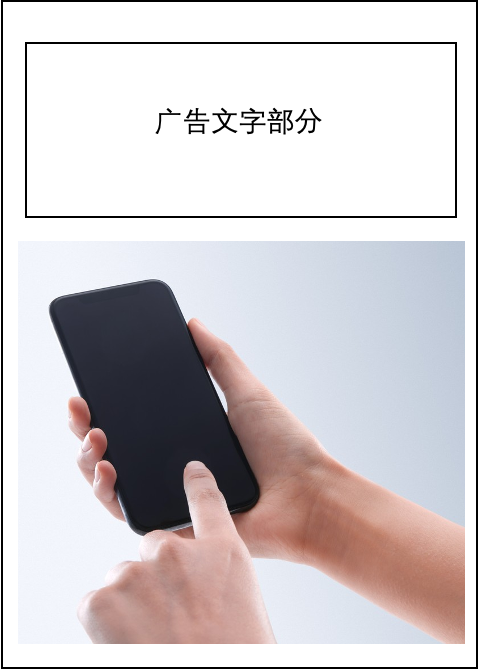
\includegraphics[width=.3\linewidth]{Image/Study2-exp1.png}
    \caption{\label{fig:Study2-exp1-ad-example}实验开始前的广告示意图}
\end{figure}

\subsection{结果}
首先分别对不同创作者(人类专家/GPT-4)生成的个性化广告效果进行检验。个性化效果通过建立人格水平与说服效果之间的线性回归模型来进行衡量,其中人格水平作为自变量,说服效果作为因变量。由于在本研究中,个性化广告是针对各人格维度的高水平个体进行设计的,因此理论上,当参与者在某一人格维度的得分越高时,相应该维度的个性化广告的说服效果越好。回归结果如下表所示(表 \ref{tab:study1_traitResults})。

结果表明,在GPT-4生成的广告中,宜人性(\textit{$\beta$} = 0.3765, \textit{p} = 0.002)、外倾性(\textit{$\beta$} = 0.1967, \textit{p} < 0.001)、尽责性(\textit{$\beta$} = 0.2978, \textit{p} < 0.001)、开放性(\textit{$\beta$} = 0.2808, \textit{p} = 0.001)四个维度上表现出人格水平对说服效果的显著正向预测效果,即宜人性/外倾性/尽责性/开放性水平越高的参与者,针对各维度高水平设计的广告说服效果更好。而神经质表现出显著相反的趋势(\textit{$\beta$} = -0.2479, \textit{p} < 0.001),即神经质水平越低越喜欢针对高神经质设计的广告。

在人类专家生成的广告中,仅宜人性(\textit{$\beta$} = 0.2685, \textit{p} = 0.004)和开放性(\textit{$\beta$} = 0.2399, \textit{p} = 0.016) 两个维度上表现出人格水平对说服效果的显著正向预测效果,即宜人性/开放性水平越高的参与者,针对各维度高水平设计的广告说服效果更好。外倾性维度上正向预测效果达到边缘显著水平(\textit{$\beta$} = 0.1343, \textit{p} = 0.087),尽责性人格水平呈正向预测效果但不显著(\textit{$\beta$} = 0.0932, \textit{p} = 0.229),而神经质人格水平的预测效果呈负向但不显著(\textit{$\beta$} = -0.1176, \textit{p} = 0.12)。

为进一步探讨人类专家与GPT-4在个性化广告创作水平上的差异,本研究对两类创作者回归斜率的差异进行了显著性检验。结果表明仅在尽责性维度上,人类专家与GPT-4的个性化水平之间差异达到边缘显著水平(\textit{t}(318) = 1.8128, \textit{p} = 0.07),具体而言,GPT-4生成的广告在该维度表现出显著的个性化效果,而人类专家的个性化效果不显著;在外倾性维度上,尽管两类信息创作者表现出不一样的趋势,即GPT-4的个性化水平显著,但人类专家的个性化水平边缘显著,但两者之间的斜率差异未达到显著水平(\textit{t}(318) = 0.6486, \textit{p} = 0.52);在宜人性(\textit{t}(318) = 0.7245, \textit{p} = 0.47)和开放性(\textit{t}(318) = 0.3115, \textit{p} = 0.76)维度上,GPT-4和人类专家在生成的个性化广告效果均显著,但两者之间不存在显著差异;在神经质维度,尽管两者存在一定的差异,但仍未达到显著水平(\textit{t}(318) = 1.4269, \textit{p} = 0.15)。

\FloatBarrier % 防止表格与正文之间的分离,强制插入位置

% \begin{table}[H]
%     \centering
%     \caption{\label{tab:study1_traitResults} 人格特质回归分析结果}
%     {\tablesongti % 整个表格环境应用宋体六号字体
%     \renewcommand{\arraystretch}{1} % 调整行距
%     \begin{tabularx}{\linewidth}{>{\raggedright\arraybackslash}X X c c c c c c}
%         \toprule
%         个性化特质 & 信息创作者 & 系数 & 标准误差 & \textit{t} & \textit{P} $>|t|$ & [0.025 & 0.975] \\ 
%         \midrule
%         \textbf{宜人性}   & \textbf{人类专家}  & 0.2685 & 0.0930 & 2.8860\textsuperscript{**} & 0.004   & 0.0848 & 0.4522 \\
%         \textbf{宜人性}   & \textbf{GPT-4}   & 0.3765 & 0.1166 & 3.2296\textsuperscript{**} & 0.002   & 0.1463 & 0.6068 \\
%         外倾性    & 人类专家   & 0.1343 & 0.0781 & 1.7206\textsuperscript{\dag} & 0.087   & -0.0198 & 0.2884 \\
%         \textbf{外倾性}    & \textbf{GPT-4}     & 0.1967 & 0.0562 & 3.5003\textsuperscript{***} & <0.001  & 0.0857 & 0.3077 \\
%         神经质     & 人类专家      & -0.1176 & 0.0752 & -1.5647 & 0.120   & -0.2661 & 0.0308 \\
%         \textbf{神经质}     & \textbf{GPT-4} & -0.2479 & 0.0518 & -4.7842\textsuperscript{***} & <0.001  & -0.3502 & -0.1455 \\
%         尽责性 & 人类专家  & 0.0932 & 0.0771 & 1.2080 & 0.229   & -0.0591 & 0.2455 \\
%         \textbf{尽责性} & \textbf{GPT-4}  & 0.2978 & 0.0825 & 3.6116\textsuperscript{***} & <0.001  & 0.1350 & 0.4607 \\
%         \textbf{开放性}        & \textbf{人类专家}        & 0.2399 & 0.0987 & 2.4309\textsuperscript{*} & 0.016   & 0.0450 & 0.4348 \\
%         \textbf{开放性}        & \textbf{GPT-4}         & 0.2808 & 0.0866 & 3.2407\textsuperscript{**} & 0.001   & 0.1097 & 0.4519 \\
%         \bottomrule
%     \end{tabularx}
%     }
%     % \vspace{1mm}
%     \caption*{\raggedright \footnotesize 注:*** $p < 0.001$,** $p < 0.01$,* $p < 0.05$,\textsuperscript{\dag} $p < 0.1$。}
% \end{table}

\begin{table}[H]
    \centering
    \caption{\label{tab:slope_difference} 不同创作者的回归斜率差异}
    {\tablesongti
    \renewcommand{\arraystretch}{1.2} % 调整行距
    \begin{tabularx}{\linewidth}{>{\centering\arraybackslash}p{3cm} >{\centering\arraybackslash}p{4cm} >{\centering\arraybackslash}p{4cm} >{\centering\arraybackslash}p{4cm}} % 居中对齐
        \toprule
        \textbf{特质} & \textbf{人类专家 (系数 \& }\textit{p}\textbf{ 值)} & \textbf{GPT-4 (系数 \& }\textit{p}\textbf{ 值)} & \textit{t 值 \& p 值} \\ 
        \midrule
        \textbf{宜人性}   & 0.2685 (0.004**)  & 0.3765 (0.002**)  & -0.7245 (0.47) \\
        \textbf{外倾性}   & 0.1343 (0.087\textsuperscript{\dag})  & 0.1967 (<0.001***)  & -0.6486 (0.52) \\
        \textbf{神经质}   & -0.1176 (0.120)  & -0.2479 (<0.001***)  & 1.4269 (0.15) \\
        \textbf{尽责性}   & 0.0932 (0.229)  & 0.2978 (<0.001***)  & -1.8128 (0.07\textsuperscript{\dag}) \\
        \textbf{开放性}   & 0.2399 (0.016*)  & 0.2808 (0.001**)  & -0.3115 (0.76) \\
        \bottomrule
    \end{tabularx}
    }
    \caption*{\raggedright \footnotesize 注:*** \textit{p} < 0.001,** \textit{p} < 0.01,* \textit{p} < 0.05,\textsuperscript{\dag} \textit{p} < 0.1。}
\end{table}






\section{实验2:引入AI修改专家内容的个性化广告效果}
实验1主要检验了GPT-4独立生成的针对大五人格高水平个体的个性化广告文案的效果,并与人类专家生成文案进行了比较。这一实验对AI生成个性化广告的潜在优势和局限性进行了初步评估。然而,实验1的研究设计在以下方面仍存在改进空间:

(1)人格测量工具的选择:实验1采用了BFI-10量表对参与者的人格特质进行测量,尽管简洁高效,但量表维度较短可能影响测量的精确性与信度。本实验改用BFI-44量表,以提升测量的标准化与可靠性,从而更全面地捕捉参与者的人格特质。

(2)因变量的设置:实验1的测量指标主要集中在广告的说服效果上,而忽略了广告在实际社交媒体场景中的潜在影响。为弥补这一不足,本实验在设计中新增了更加贴近实际应用的因变量,包括「支付金额」和「微博交互行为意愿程度」,以更全面地评估个性化广告的效果。

(3)人机协作情境的考察:实验1仅比较了GPT-4独立生成文案与人类专家生成文案的效果,未涉及AI与人类专家合作的情境。然而,在实际广告创作中,人机协作是AI技术应用的重要方向。为探讨GPT在辅助人类专家优化广告文案中的潜力,本实验新增了GPT对人类专家生成文案的修改组(即GPT-loop),以进一步评估GPT在协作场景下对广告文案效果的影响。

\subsection{方法}
根据上述调整,本实验采用 \textbf{3(信息创作者:AI/人类专家/AI修改专家)}的被试间设计。AI和人类专家条件与实验1保持一致 \ref{实验1:GPT-4与人类专家在不同人格特质广告生成中的比较},AI修改专家组为新增条件,在专家生成的文本基础上,引导AI对文案进行优化和调整。个性化条件与实验1一致,针对五种不同人格水平(外倾性、开放性、尽责性、宜人性、神经质)的高水平特质进行个性化设计,即分别为高外倾、高开放、高尽责、高宜人和高神经质的消费者设计了广告内容。

\textbf{(1)被试}

通过见数平台发布实验,378名参与者自愿参加这项研究。10名参与者由于注意检查测试未通过被剔除,剩余\textbf{368}名有效被试(年龄范围= 18-56岁;\textit{M}=25.70岁;\textit{SD}=6.63;女性228名)。参与任务的每名参与者获得5元人民币作为报酬。注意力检测题设置为人格测试中的一致性验证题,采用BFI-44量表中的原题和逆向表述的对比形式。具体而言,将BFI-44量表中的原题“我是健谈的”设置为其反向表述形式“我不是健谈的”。若参与者在这两道题目上的评分一致,且均不为中间分值(即3分),则被视为通过检测;否则,视为注意力检测未通过。


\textbf{(2)问卷测量}

a. 大五人格量表。采用\citet{john1991big}编制44道题目的大五人格量表(Big Five Inventory,BFI-44)测量参与者的人格特征。该量表共44个项目,分属外倾性、宜人性、神经质、开放性、尽责性5个维度。参与者在 5 点李克特式量表上进行评分(选项“1”代表“非常不符合”,“5”代表“非常符合”)。

b. 因变量。本实验设置三个因变量,分别为说服效果、微博互动意愿、支付金额。其中说服效果与实验1一致,具体测量方式详见表\ref{tab:persuasionSurvey})。微博互动意愿参考\citet{winter2021effects}的设计,通过四个题项评估参与者对广告微博可能产生的具体互动行为意愿。具体题目包括:(1)“我会点击并访问广告发布者的微博主页”;(2)“我会点赞该微博”;(3)“我会评论该微博”;(4)“我会转发/分享该微博”。参与者需基于五点李克特量表进行评分,其中“1”代表“非常低”,“5”代表“非常高”。支付金额参考\citet{matz2024potential}的方法,要求参与者对愿意为广告中的产品支付的金额进行评估,支付金额范围设置为0元至10000元人民币,具体金额区间是根据Canalys 2023年第二季度中国智能手机均价(约450美元,折合人民币3300元)合理扩展而来,旨在模拟实际消费场景。

\textbf{(3)广告材料}

针对3(信息创作者:AI/人类专家/AI修改专家)*5(广告人格:外倾性/开放性/尽责性/宜人性/神经质)共15个条件生成广告材料。广告内容的产品仍为手机,与实验1保持一致。

人类专家组的材料与实验1一致。在AI组和AI修改专家组中,广告文案则重新生成。尽管AI组在实验1中已存在,但为确保本实验中AI相关条件的一致性,AI组与AI修改专家组的文案均由相同的模型生成。在AI修改专家组中,文案生成的具体操作是基于专家组的原始文案进行改写,明确要求GPT以专家文案为基础对内容进行优化调整,而非直接生成全新的文案。每个条件生成5-6个信息,初始生成53则广告文本材料,经过预实验筛选,剩余38条(详见附录)。通过见数平台发布实验,329名参与者自愿参加预实验(年龄范围= 18-72岁;\textit{M}=30.44岁;\textit{SD}=9.35;女性200名)。每名参与者仅参与一个实验条件,即针对某一信息创作者生成的广告文案和某一人格维度设计的广告材料进行评价。每个条件下包含5-6则广告文案。参与者在阅读每则广告文案后,需根据广告面向的目标消费者特点进行评价。评分采用1-5点量表,其中1分表示更符合“低水平”描述,5分表示更符合“高水平”描述。例如,对于针对高尽责性设计的广告,参与者需基于以下特征进行评分,从“粗心的、容易分心的、不拘小节的、做事缺少条理的”到“可靠的、有组织的、自律的、注重细节的、有条理”。此外,参与者还需对广告的理解程度(即消费者是否能理解广告是在宣传手机)进行1-5点量表评分。预实验通过两个筛选条件来选择用于正式实验的实验材料: 1)广告目标消费者特点评分需大于3分;2)广告理解程度评分需大于3分。根据以上筛选标准,最终保留每个条件下2-6则广告文本材料用于正式实验,具体材料详见附录。

\subsection{实验流程}
在实验开始前,参与者被告知接下来他们将对五则社交媒体上的广告进行评价。所有广告文案的配图相同(见图\ref{fig:Study2-exp2-ad-example}),区别在于广告文案内容。为了模拟更实际的社交媒体场景,相较于实验1,本实验的广告界面增加了微博平台的视觉元素,包括虚拟的头像、虚拟的微博账号名,以及点赞、评论和转发等交互按键。参与者将依次阅读五则广告的文案,并在每阅读完一则文案后立即对其说服效果/微博参与意愿/支付金额进行评分。完成所有五则广告文案的评价后,参与者需回答与人格测试相关的问卷题目,最后提供年龄、性别等人口统计学信息。

\begin{figure}[htbp]
    \centering
    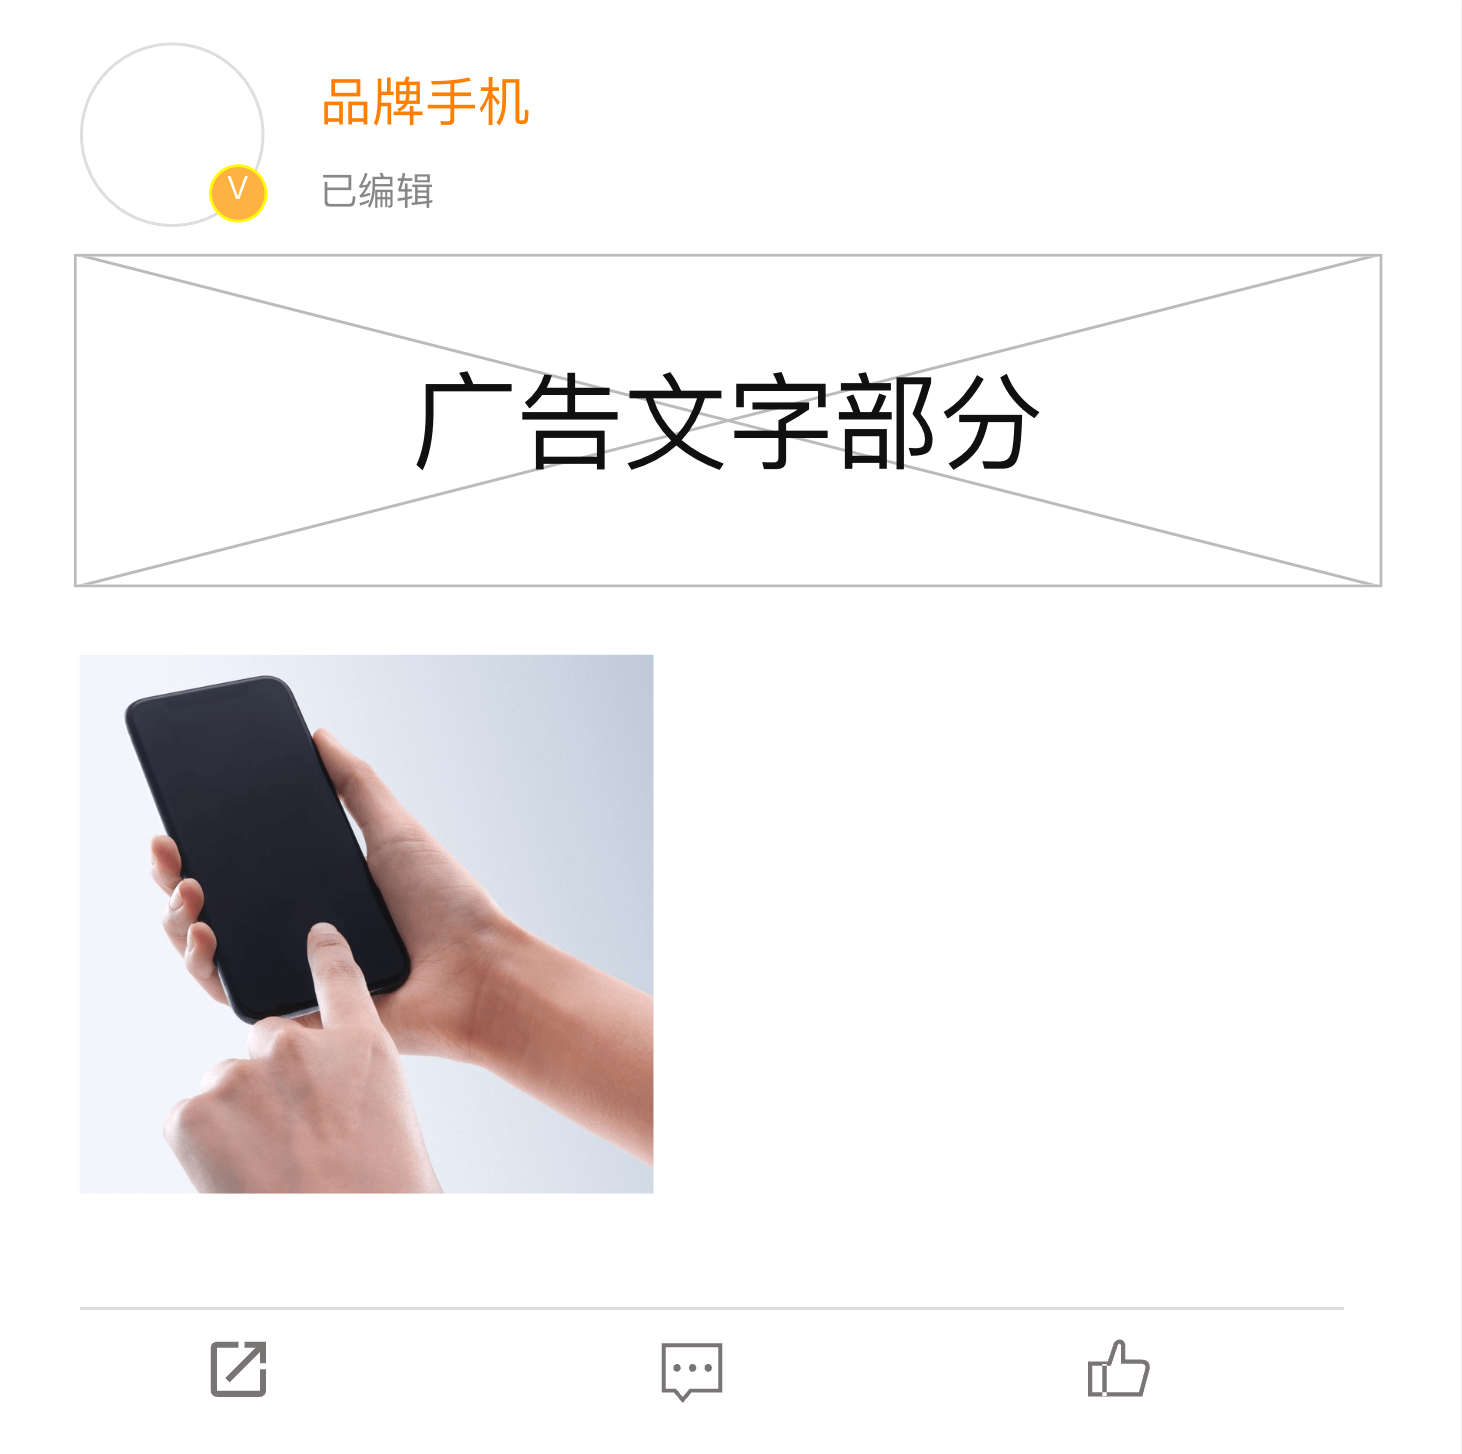
\includegraphics[width=.3\linewidth]{Image/Study2-exp2.png}
    \caption{\label{fig:Study2-exp2-ad-example}实验开始前的广告示意图}
\end{figure}


\subsection{结果}
本实验的分析方法与实验1相似,分别对不同信息创作者(人类专家/AI/AI修改专家)生成的个性化广告效果进行检验。个性化效果通过建立人格水平与因变量(说服效果、微博互动意愿、支付金额)之间的线性回归模型来衡量,其中人格水平作为自变量,三个效果指标作为因变量。由于在本实验中,个性化广告是针对各人格维度的高水平个体进行设计的,因此理论上,当参与者在某一人格维度的得分越高时,相应维度的个性化广告的效果指标应表现更好。此外,由于支付金额的范围较广(0-10000元),在分析过程中对其进行了归一化处理。

结果表明,在三个广告效果指标上,AI (GPT-4) 和 AI 修改专家组 (GPT-4 修改专家) 在宜人性、外倾性、尽责性和开放性四个维度上均表现出稳定且显著的个性化效果(回归显著,\textit{p}s < 0.05)。这说明,特质得分越高,针对高特质设计的广告效果越好,符合预期。而在神经质维度上,三个创作者的广告均表现出稳定的负向结果,即神经质得分越低,针对高神经质设计的广告效果评价越高。人类专家组在外倾性、尽责性和开放性维度上也表现出显著的个性化效果,且与 AI 组和 AI 修改专家组结果一致。但在人类专家组中,宜人性维度的个性化效果不显著(\textit{p} > 0.05)。

\begin{table}[H]
    \centering
    \caption{\label{tab:slope_difference_study2} 不同创作者的回归斜率差异(说服效果)}
    {\tablesongti
    \renewcommand{\arraystretch}{1.2} % 调整行距
    \begin{tabularx}{\linewidth}{>{\centering\arraybackslash}p{3cm} >{\centering\arraybackslash}p{4cm} >{\centering\arraybackslash}p{4cm} >{\centering\arraybackslash}p{4cm}} % 居中对齐
        \toprule
        \textbf{特质} & \textbf{人类专家 (系数 \& }\textit{p}\textbf{ 值)} & \textbf{GPT-4 (系数 \& }\textit{p}\textbf{ 值)} & \textbf{GPT-Loop (系数 \& }\textit{p}\textbf{ 值)} \\ 
        \midrule
        \textbf{外倾性}   & 0.3145 (0.002**)  & 0.3143 (0.001**)  & 0.3431 (0.001**)  \\
        \textbf{宜人性}   & 0.1270 (0.419)  & 0.4350 (0.003**)  & 0.6969 (<0.001***)  \\
        \textbf{尽责性}   & 0.3221 (0.002**)  & 0.4375 (<0.001***)  & 0.4022 (0.001**)  \\
        \textbf{神经质}   & -0.3358 (0.001**)  & -0.3423 (0.001**)  & -0.4036 (0.001**)  \\
        \textbf{开放性}   & 0.4017 (0.004**)  & 0.4859 (<0.001***)  & 0.6110 (<0.001***)  \\
        \bottomrule
    \end{tabularx}
    }
    \caption*{\raggedright \footnotesize 注:*** \textit{p} < 0.001,** \textit{p} < 0.01,* \textit{p} < 0.05,\textsuperscript{\dag} \textit{p} < 0.1。}
\end{table}


进一步,我们比较了三类信息创作者在回归斜率上的显著性差异。结果表明,仅在宜人性维度上,AI 修改专家组与人类专家组在说服效果(\textit{t} = 2.66,\textit{p} = 0.008)和微博互动意愿(\textit{t} = 1.96,\textit{p} = 0.05)两个指标上表现出显著差异。人类专家组本身的个性化效果不显著,而 AI 和 AI 修改专家组的个性化效果显著且稳定。同时,显著性差异检验表明 AI 修改专家组显著优于人类专家组。这一结果说明,GPT-4 在优化人类专家文案时能够显著提升宜人性维度广告的效果。此外,与实验1相比,人类专家组在宜人性维度上的表现发生了变化:实验1中,人类专家组的宜人性个性化效果显著,而本实验中则未达到显著性水平。为探讨这一差异,本研究分析了实验1和本实验所使用的人格测量工具(BFI-10 和 BFI-44)的相关性(如图\ref{fig:study2-correlation})。结果显示,宜人性维度的相关性较低(0.67),而其他四个维度的相关性均较高(>0.80)。这表明,本实验中使用的 BFI-44 测量工具具有更高的精确度和可靠性,因此本实验的结果更可信。此外,在实验1中,人类专家组在外倾性和尽责性维度上未表现出显著的个性化效果,但在本实验中,这两个维度的效果变得更显著。结合测量工具的改进,可以推测,使用更精细的量表后,外倾性和尽责性维度的个性化效果更加稳定。

\begin{figure}[H]
    \centering
    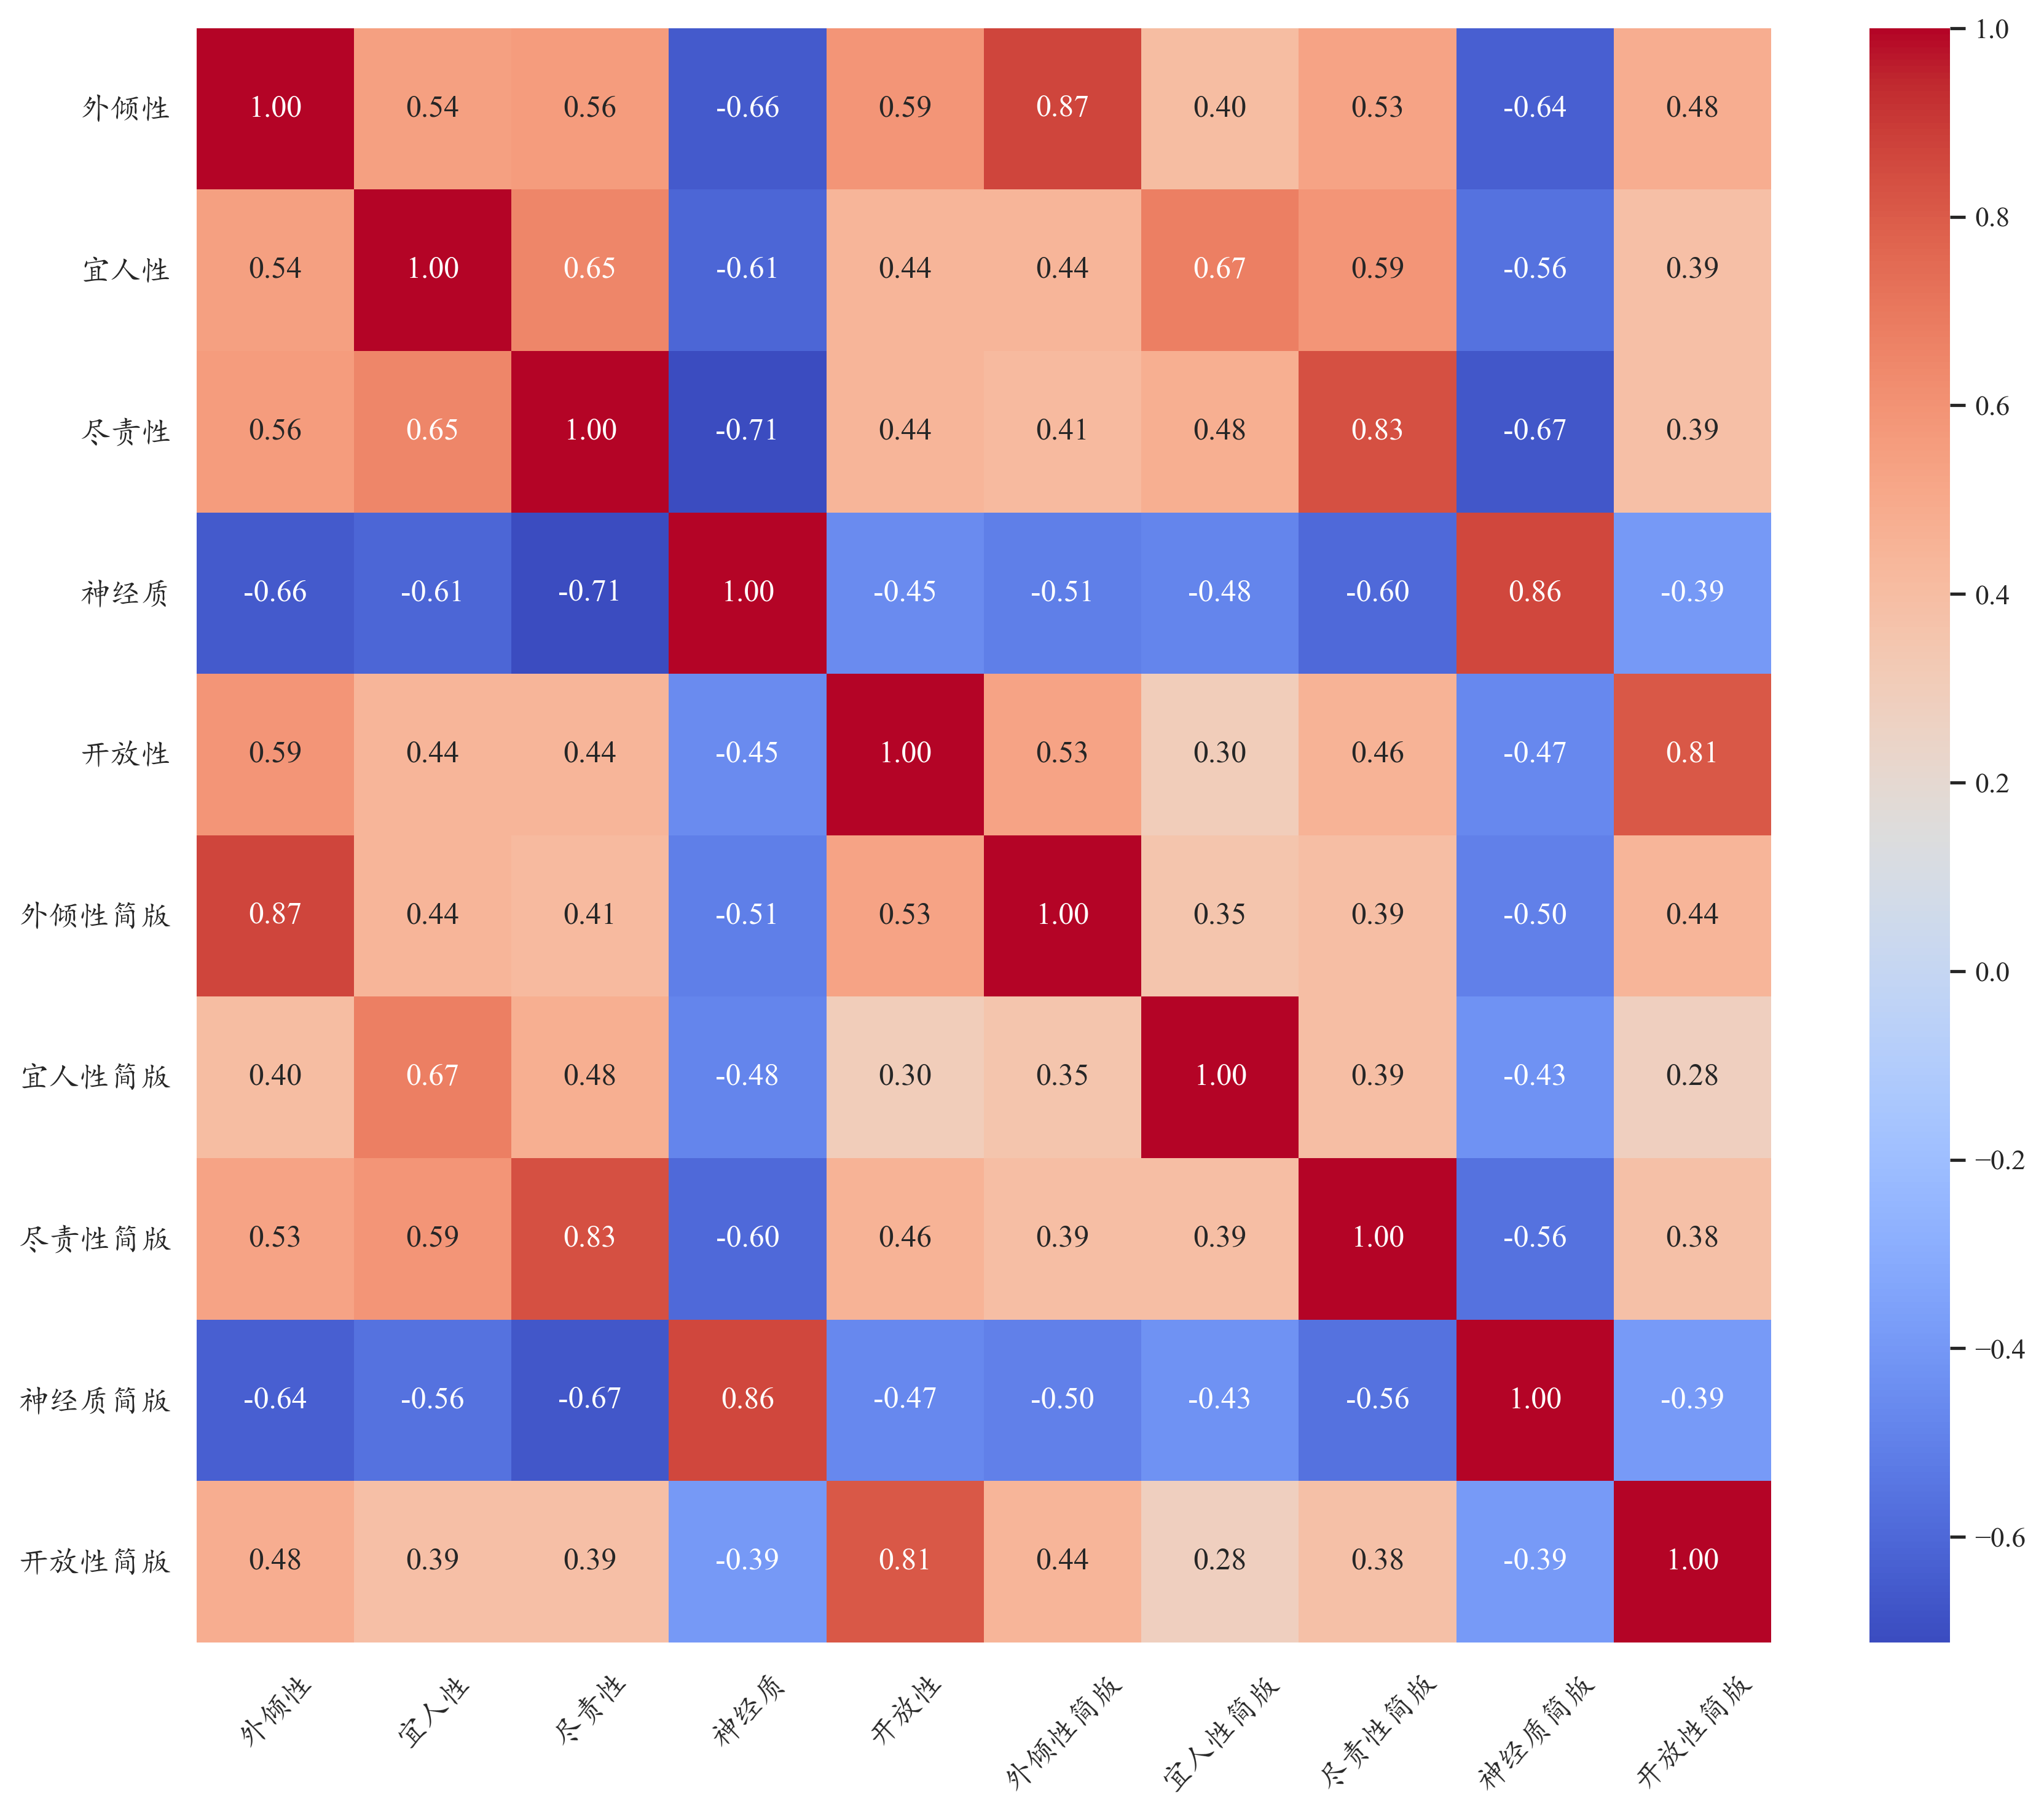
\includegraphics[width=1\linewidth]{Image/BFI44-BFI10相关.png}
    \caption{\label{fig:study2-correlation}BFI44-BFI10相关}
\end{figure}

神经质维度的负向结果表现出一致性。以说服效果为例,AI组(\textit{$\beta$} = -3.410, \textit{p} < 0.01),人类专家组(\textit{$\beta$} = -3.441, \textit{p} < 0.01),AI修改专家组(\textit{$\beta$} = -3.571, \textit{p} < 0.01)在神经质维度上均呈现显著负向预测趋势,即神经质得分较低的个体对针对高神经质设计的广告评价更高。这一结果与前人研究中提到神经质的特殊性一致\citep{matz2024potential}。这一现象的机制可能与高神经质广告传递的情感特征有关,后续研究将进一步结合对 AI 生成广告特征的内容分析进行深入探讨。

综上所述,本实验的结果表明,AI 和 AI 修改专家组在宜人性、外倾性、尽责性和开放性维度上均表现出显著且稳定的个性化效果,而人类专家组在宜人性维度上的表现不如预期,但在外倾性、尽责性和开放性维度上仍显示出一定能力。特别是AI修改专家组在宜人性维度上的显著提升,进一步证明 AI 技术不仅能够独立生成高效的个性化广告,还可以通过与人类专家协作进一步优化广告内容,从而为个性化广告设计中的人机协作提供重要启示。





\section{讨论}

本研究通过实验1和实验2系统地比较了AI(GPT-4)与人类专家在个性化广告创作中的表现,并进一步探讨了AI优化人类专家广告文案的潜力。结果表明,AI能够在多个人格特质维度上生成有效的个性化广告,且在某些特质(如尽责性)上,其个性化效果甚至优于人类专家。此外,当AI用于优化人类专家文案时,个性化广告的效果在宜人性维度得到了显著提升。这一发现不仅为AI在个性化广告领域的应用提供了新的证据,也为更广泛的说服与信息传播研究提供了重要启示 \citep{dehnert2022persuasion}。

尽责性和宜人性两个特质的个性化广告在实验结果中展现出了一定的复杂性。在尽责性维度上,GPT-4 生成的广告表现出稳定的个性化匹配效果,而人类专家的个性化效果则不显著,且GPT-4和人类专家的效果在实验1中存在边缘显著的差异。这一结果表明,AI在尽责性个性化广告的创作上具有更强的适配性,而人类专家在这一维度的广告效果则存在较大的不确定性。尽责性人格的核心特征包括自律、责任感和条理性\citep{roberts2014conscientiousness},这类个体通常偏好结构清晰、信息明确、逻辑严谨的广告内容。然而,人类专家在撰写广告时可能受到自身写作风格的影响,使得广告文本在逻辑性和条理性上存在个体差异,导致尽责性个性化广告的效果不稳定。而GPT-4 作为基于大规模语料训练的AI模型,能够在生成过程中更一致地遵循逻辑清晰、信息直接的模式,因此其尽责性个性化广告更具稳定性。这也说明,通过优化prompt以及随着模型能力的提升,AI在尽责性个性化广告创作中的适应性可能仍在增强。

在宜人性维度上,实验2的结果显示,GPT-4 修改人类专家文案后,其个性化广告在说服效果和微博互动意愿方面均显著优于人类专家组,而人类专家组本身的个性化效果未达到显著水平。这一发现表明,在宜人性个性化广告的创作过程中,AI不仅能够独立生成有效的个性化广告,还能够优化人类专家的广告,使其更符合目标受众的需求。宜人性人格的个体通常更加注重社交互动、合作与温暖的表达\citep{graziano2007agreeableness},这意味着个性化广告需要更强的情感共鸣和人际取向。然而,人类专家可能并未能充分把握宜人性个体的偏好,导致其广告在实验间表现出较大的不稳定性。而AI在优化人类专家广告时,能够更系统性地强化广告中的情感元素和亲和力表达,使其更符合高宜人性个体的预期。这表明,在个性化广告创作中,AI不仅能够弥补人类专家可能存在的个性化表达不足,还能够通过文本优化进一步提升广告的个性化适配度。

另一方面,在神经质维度上,实验1和实验2均未能发现预期的个性化效果,且在实验2中,所有创作者的广告均表现出稳定的负向匹配效应,即神经质水平较低的个体对针对高神经质设计的广告评价更高。这一现象可能表明,神经质个体在广告偏好上的特征较为特殊,并不容易通过传统的个性化匹配策略进行有效优化。一个可能的解释是,高神经质个体通常具有较高的焦虑和不安全感,因此他们可能更倾向于接受带有安抚性、稳定性描述的广告,而不是直接迎合其负面情绪特征的广告。而低神经质个体可能对“高神经质广告”中涉及的情绪化表达、焦虑驱动的语言特征更敏感,甚至产生更强的情绪共鸣,从而导致负向匹配效应的出现。此外,高神经质个体可能对广告信息的解读方式不同于低神经质个体,他们更容易受到信息的情绪基调和潜在风险暗示的影响这可能进一步导致高神经质个体对高神经质广告的接受度较低,而低神经质个体则因广告的情绪化特征反而产生更高的评价。这一发现提示,在未来的个性化广告优化中,需要更深入地探讨神经质个体对广告内容的具体偏好模式,以避免简单的人格匹配策略在这一特质上的局限性。

尽管研究一和研究二验证了AI在个性化广告创作中的有效性,并探索了其与人类专家在个性化匹配效果上的差异,但这些实验的分析主要基于参与者被试的行为反馈,而未能深入解析广告文本本身的特征。特别是在尽责性和宜人性维度,AI展现出更稳定且更优的个性化匹配能力,而人类专家创作的广告则表现出较大的不确定性,这一结果表明,个性化广告的效果不仅受到受众人格特质的影响,也可能取决于广告文本本身的语言模式。然而,目前的实验结果仍未能清楚地揭示个性化广告创作中所采用的文本特征究竟存在何种系统性的差异,以及这些文本特征如何影响受众对广告的接受度。因此,仅通过参与者评分来判断个性化广告的有效性仍然是不够的,进一步的文本分析有助于揭示广告文本本身的结构、内容以及语言特征如何与不同人格特质的受众需求相匹配。在个性化广告研究中,文本特征的作用往往难以被系统地研究,因为传统的广告文本数量较少,难以进行规模化的文本分析。然而,AI的快速生成能力使得本研究能够积累大量的个性化广告文本及其参与者评分数据,从而为文本特征的深入分析提供了可能性。研究三将在研究一和研究二的基础上,结合大规模文本数据,系统地分析个性化广告文本在不同人格特质维度上的语言模式,并构建预测模型,以识别最能影响个性化广告说服效果的关键特征。这不仅能够帮助我们更好地理解AI在个性化广告创作中的优势与局限,也能为未来的人机协作广告创作提供数据驱动的优化策略,从而推动个性化广告生成技术的进一步发展。


